\documentclass[tikz]{standalone}
\usetikzlibrary{positioning,calc}

\begin{document}
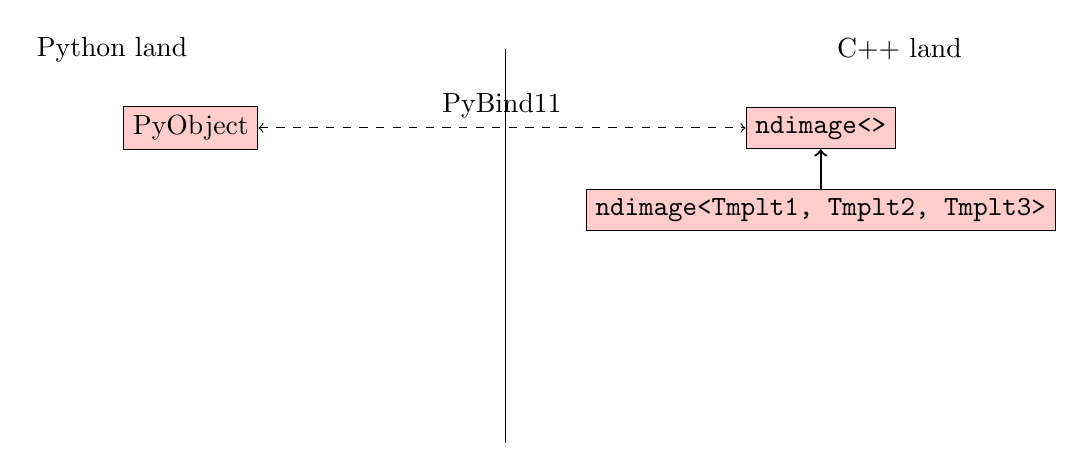
\begin{tikzpicture}
\tikzset{land/.style={draw}, obj/.style={draw,fill=red!20}};
   \draw node[] (A) {Python land} -- ++(10,0) node[] (B) {C++ land};
   \coordinate (C)  at ($(A)!0.5!(B)$);
   \draw (C) -- ++(0,-5);

   \node[obj] at (1, -1) (Py0) {PyObject};
   \node[obj] at (9, -1) (A) {\tt ndimage<>};
   %\node[obj] [below = 0.5cm of A] (B) {\tt ndimage<Tmplt1>};
   %\node[obj] [below = 0.5cm of B] (C) {\tt ndimage<Tmplt1, Tmplt2>};
   \node[obj] [below = 0.5cm of A] (D) {\tt ndimage<Tmplt1, Tmplt2, Tmplt3>};

   \draw[<->,dashed] (Py0) -- (A) node[midway,above] {PyBind11};
    %\draw[->,thick] (B) -- (A)  node[midway,above] {};
    %\draw[->,thick] (C) -- (B)  node[midway,below] {};
    \draw[->,thick] (D) -- (A)  node[midway,above] {};

\end{tikzpicture}
\end{document}
